\documentclass[11pt, aspectratio=169]{beamer}

% ── Theme ──────────────────────────────────────────────────────────────────────
\usetheme{metropolis}
\usepackage[utf8]{inputenc}
\usepackage[T1]{fontenc}
\usepackage[english]{babel}
\usepackage{lmodern}
\usepackage{graphicx}
\usepackage{booktabs}
\usepackage{tabularx}
\usepackage{tikz}

\graphicspath{{../figures/}{figures/}}

% ── Colors (same as docs/rapport_specification.tex) ─────────────────────────────
\definecolor{ritsu}{RGB}{0, 75, 135}
\setbeamercolor{palette primary}{bg=ritsu, fg=white}
\setbeamercolor{titlelike}{fg=ritsu}
\setbeamercolor{progress bar}{fg=ritsu, bg=ritsu!20}
\setbeamercolor{frametitle}{bg=ritsu}

\setbeamertemplate{frame footer}{Raphael BELY --- DDSE Lab, Ritsumeikan}

% ── Visible placeholder for the skeleton (replace before the talk) ─────────────
\newcommand{\todonote}[1]{{\color{gray}\itshape [TO COMPLETE --- #1]}}

% ── Metadata ─────────────────────────────────────────────────────────────────
\title{Error Pattern Analysis in an Online Judge System}
\subtitle{Reproducing and Extending Shimizu et al. (2025)}
\author{Raphael BELY}
\institute{DDSE Laboratory --- Ritsumeikan University}
\date{August 28, 2026}
\titlegraphic{%
  
\includegraphics[width=2.6cm,height=1.1cm,keepaspectratio]{logo_ritsumeikan.png}\hfill
  
\includegraphics[width=2.2cm,height=0.85cm,keepaspectratio]{logo_em.jpg}%
}

\begin{document}

\maketitle

% ═══════════════════════════════════════════════════════════════════════════
\begin{frame}{About This Internship}
  \begin{minipage}{0.76\textwidth}
    \begin{itemize}
      \item Research internship --- DDSE Laboratory, Ritsumeikan University
      \item Supervised by Prof. Makihara Erina
      \item Goal: reproducing, then extending\\
        {\small\emph{Shimizu, Makihara \& Yoshida (2025) --- An Empirical
        Study of the Error Characteristics in an Online Judge System, FSE
        Companion '25.}}
      \item May 28 -- September 20, 2026 (16 weeks)
      \item French student, Enseirb-Matmeca (Bordeaux INP) --- 4-year
        engineering program, 1 year left after this, AI specialization
    \end{itemize}
  \end{minipage}
  \begin{tikzpicture}[remember picture, overlay]
    \node[anchor=south east, xshift=-0.7cm, yshift=0.7cm] at (current page.south east) {
      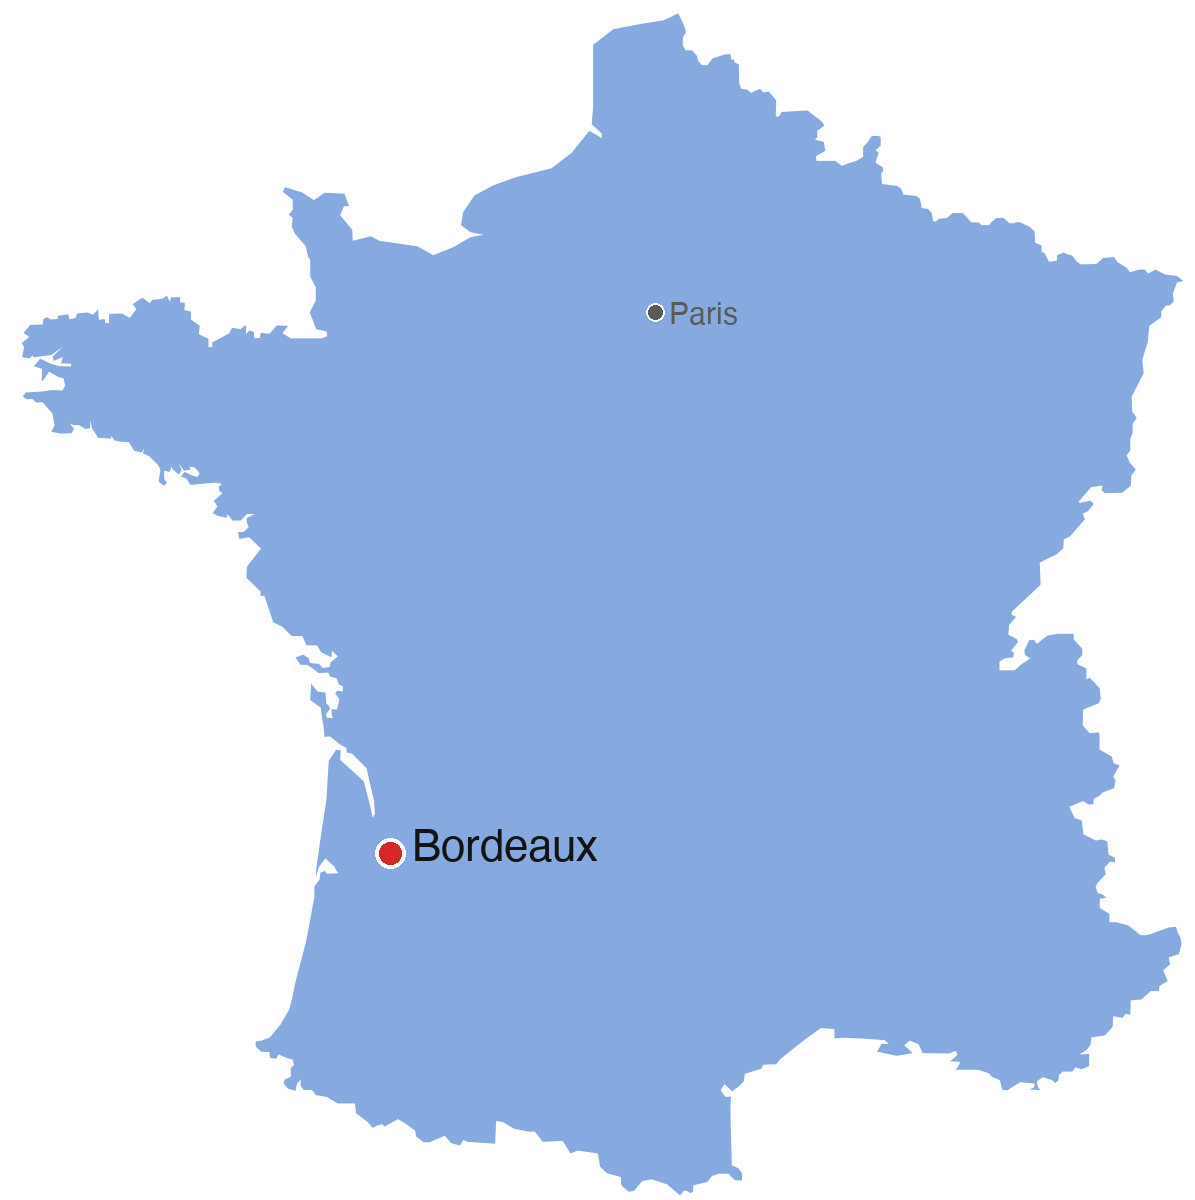
\includegraphics[width=2.6cm]{france_bordeaux_map.png}
    };
  \end{tikzpicture}
\end{frame}

% ═══════════════════════════════════════════════════════════════════════════
\section{The Dataset}

\begin{frame}{Project CodeNet}
  \begin{itemize}
    \item IBM Research (2021) --- built by scraping two online judges:
      \textbf{AIZU} and \textbf{AtCoder}
    \item Official CodeNet total (both sources combined): 4,053 problems,
      13,916,868 submissions\\
      {\tiny\color{gray} Puri et al. 2021, arXiv:2105.12655}
    \item \textbf{This project analyzes}: the AtCoder side only, restricted
      to ABC contests --- 659 problems (difficulty A--F), \textasciitilde
      8.9M submissions, 96,207 users
    \item One file = one submission, path encodes everything:\\
      \small\texttt{data/(problem\_id)/(language)/(submission\_id).ext}\\
      \small e.g. \texttt{data/p00023/C++/s006384060.cpp}
  \end{itemize}
\end{frame}

\begin{frame}{What We Measure}
  \begin{columns}[T]
    \column{0.5\textwidth}
    \textbf{Submission verdict}
    \begin{itemize}
      \item AC --- Accepted
      \item WA --- Wrong Answer
      \item TLE --- Time Limit Exceeded
      \item RE --- Runtime Error
      \item CE --- Compile Error
    \end{itemize}
    \vspace{1mm}
    \textbf{Also tracked}: problem difficulty, A (easy) $\to$ F (hard)
    \vspace{1mm}\\
    \small \textbf{One real row, same order as the file path above:}\\
    problem \texttt{p02659} (C) $\to$ Python $\to$ \texttt{s718190921}
    $\to$ \textcolor{red!70!black}{WA} \textbf{+ code}
    \column{0.44\textwidth}
    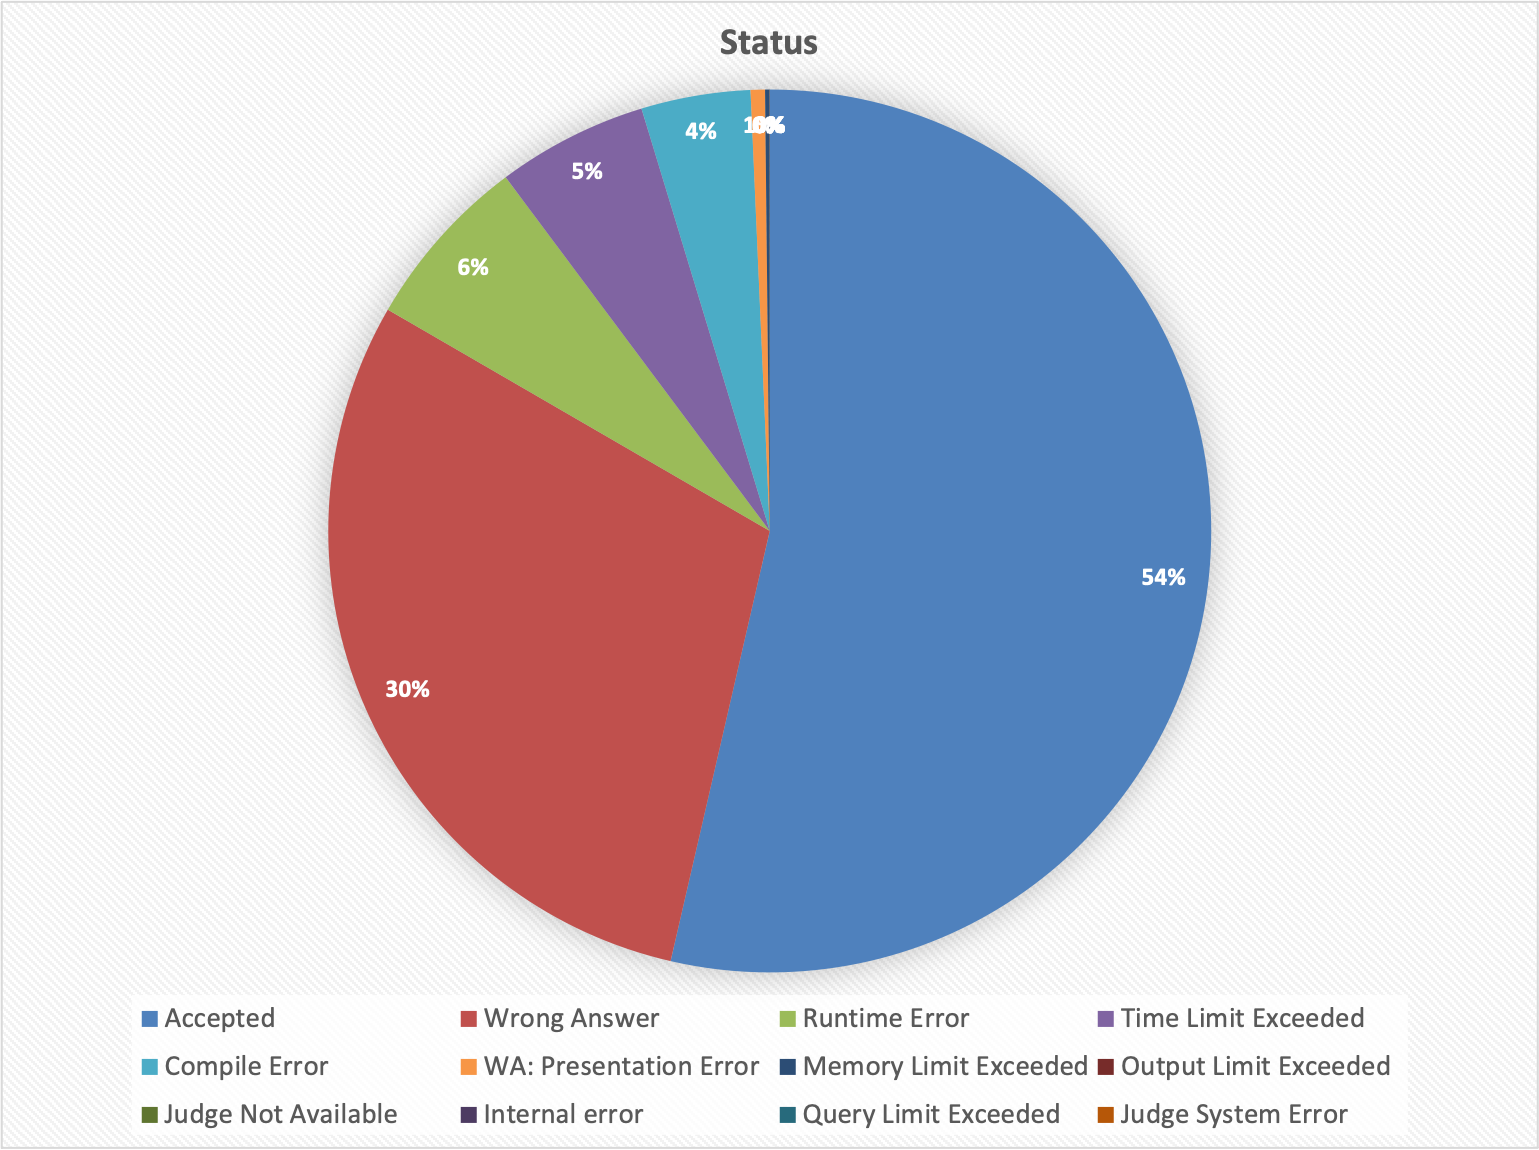
\includegraphics[width=\linewidth]{codenet_official_langs_status.png}\\
    {\tiny\color{gray} Official CodeNet-wide verdict breakdown (Puri et al.
    2021, arXiv:2105.12655) --- all languages/sources pooled, not just our
    AtCoder/Python subset.}
  \end{columns}
\end{frame}

% ═══════════════════════════════════════════════════════════════════════════
\section{Research Questions}

\begin{frame}{RQ1, RQ2, RQ3}
  \begin{block}{RQ1 --- Error Patterns}
    How do programmers' error patterns vary with problem difficulty and user
    proficiency?
  \end{block}
  \begin{block}{RQ2 --- Code-Level Semantic Analysis}
    Do codes that are close together in vector space share the same error
    pattern?
  \end{block}
  \begin{block}{RQ3 --- Prediction (optional)}
    Can RQ1/RQ2 insights function as a predictive model? --- still open,
    this is what the post-Aug-28 LLM exploration will test
  \end{block}
\end{frame}

% ═══════════════════════════════════════════════════════════════════════════
\section{Methodology}

\begin{frame}{General Approach}
  \begin{itemize}
    \item \textbf{RQ1}: classify users (G1--G6), then cross-tabulate error
      rates by difficulty
    \item \textbf{RQ2}: embed code, test whether neighbors in that space
      share the same verdict
    \item \textbf{The rule behind every number in this talk}: never report
      one in isolation --- always against a reference (a random baseline,
      chance, or Shimizu's own numbers)
  \end{itemize}
\end{frame}

% ═══════════════════════════════════════════════════════════════════════════
\section{Results --- RQ1}

\begin{frame}{Reminder: RQ1}
  \begin{center}
    \Large How do programmers' error patterns vary with problem
    difficulty and user proficiency?
  \end{center}
\end{frame}

\begin{frame}{Preliminary --- G1--G6 Classification}
  \begin{columns}[T]
    \column{0.5\textwidth}
    \begin{itemize}
      \item \textbf{Question}: can users be sorted into meaningful
        proficiency groups?
      \item Not a CodeNet field --- this is \textbf{step 1 of Shimizu's
        method}, reproduced here first
      \item \textbf{Method}: group = hardest difficulty ever solved
      \item \textbf{Result}: monotonic trends G1$\to$G6 --- win rate
        76.8\%$\to$95.8\% --- validated against Shimizu Table 3 (+6--8\%
        gap, explained)
    \end{itemize}
    \column{0.48\textwidth}
    \centering
    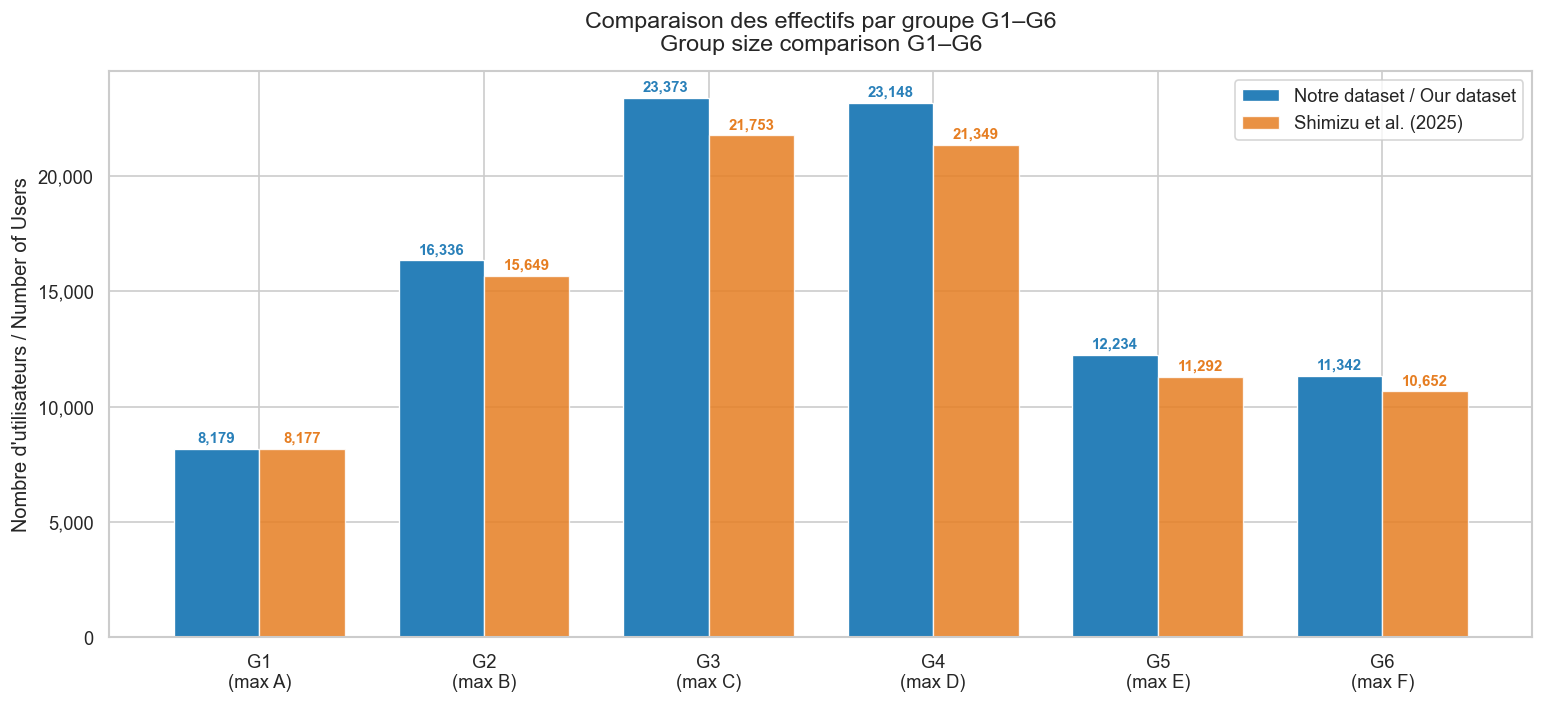
\includegraphics[height=3.1cm]{nb01_g1g6_vs_shimizu.png}\\[1mm]
    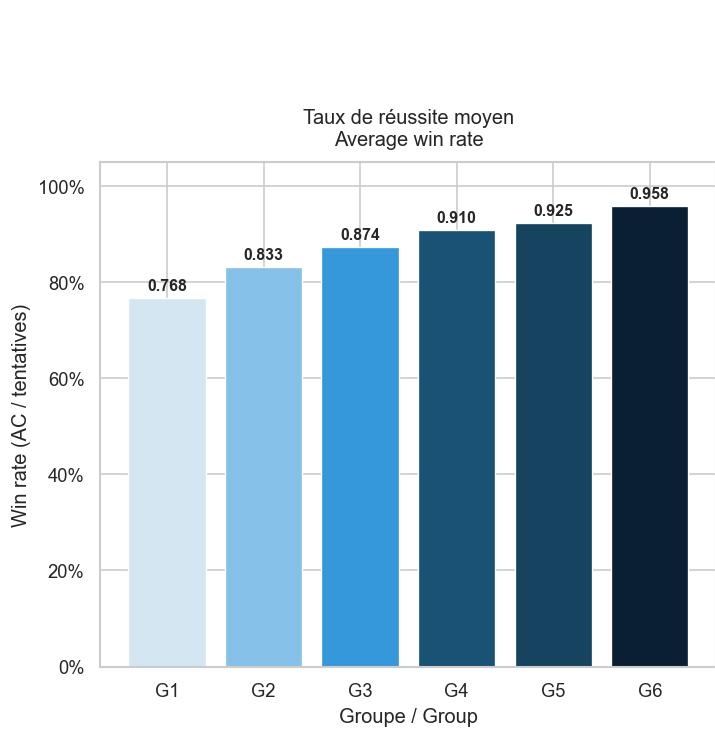
\includegraphics[height=3.1cm]{nb01_winrate_panel.png}
  \end{columns}
\end{frame}

\begin{frame}{Quick Detour: Language Matters --- Not as Expected}
  \begin{columns}[T]
    \column{0.52\textwidth}
    \begin{itemize}
      \item \textbf{Question}: does language choice influence the error
        type?
      \item \textbf{Result 1}: TLE $\sim$3$\times$ more frequent in Python
        than C++ (23.2\% vs 8.2\%, level D)
      \item \textbf{Result 2 (counter-intuitive)}: beginners (G1) do
        \alert{not} mostly use Python --- 54.3\% in C++
    \end{itemize}
    \column{0.44\textwidth}
    \centering
    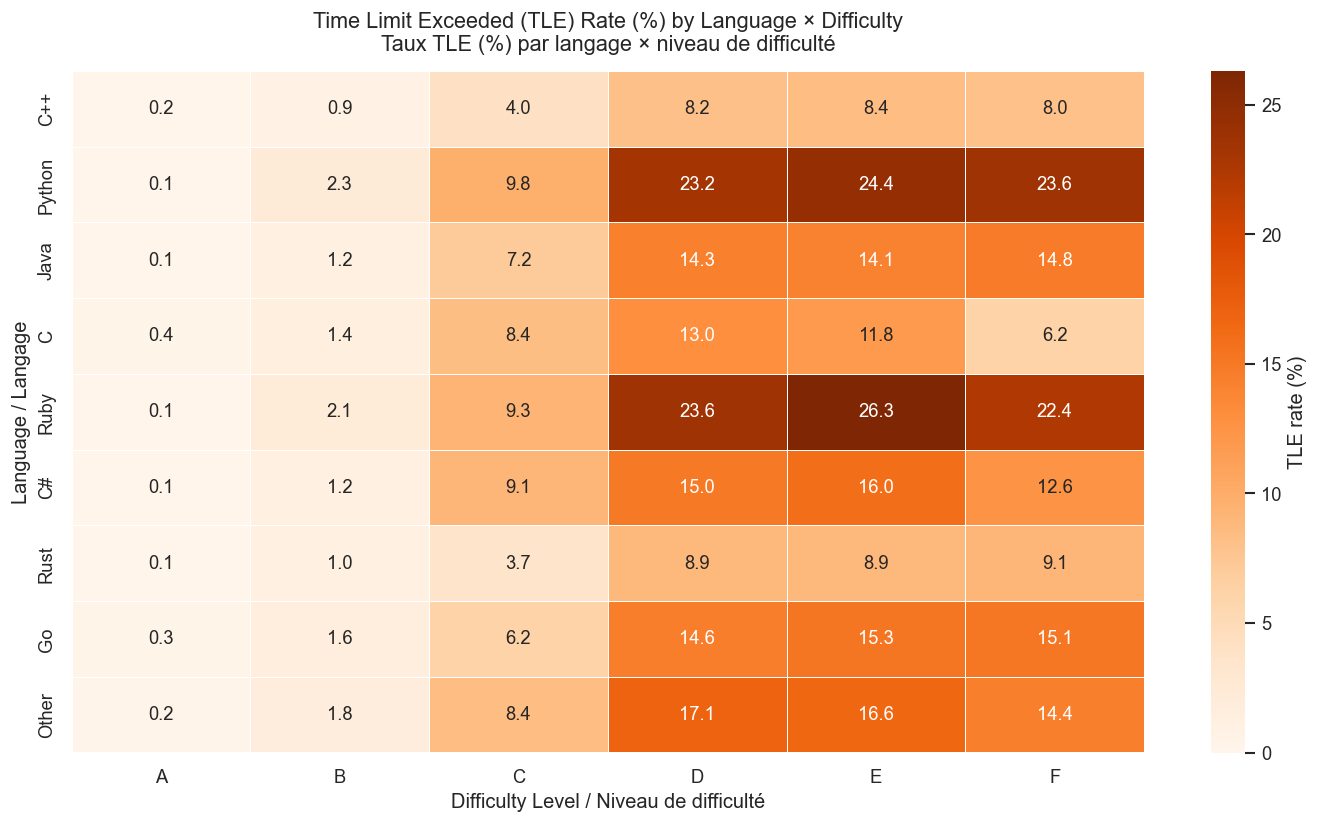
\includegraphics[height=3.1cm]{nb04_tle_by_language.png}\\[1mm]
    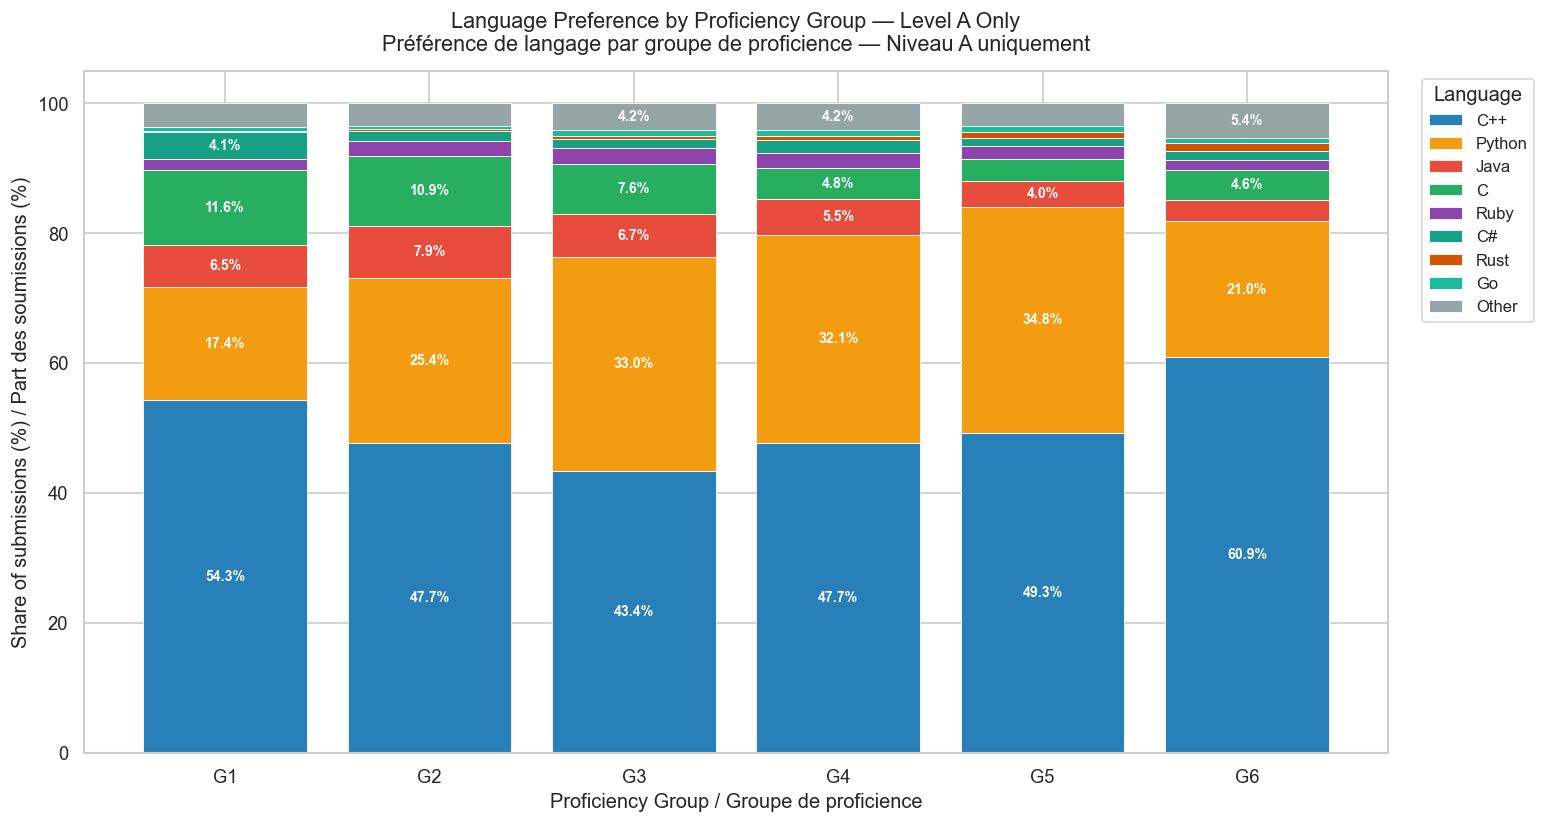
\includegraphics[height=3.1cm]{nb04_language_by_group.png}
  \end{columns}
\end{frame}

\begin{frame}{Validation \& Persistence}
  \begin{columns}[T]
    \column{0.48\textwidth}
    \textbf{CE$\leftrightarrow$TLE inversion}
    \begin{itemize}
      \item AC rate: 73\%$\to$35\% (A$\to$F)
      \item Replicates Shimizu Figure 4
    \end{itemize}
    \vspace{2mm}
    \textbf{Resolution \& first try}
    \begin{itemize}
      \item Resolution: 98.1\%$\to$80.5\% (A$\to$F)
      \item First-try AC falls faster: 81.0\%$\to$39.1\% (A$\to$F)
    \end{itemize}
    \column{0.48\textwidth}
    \centering
    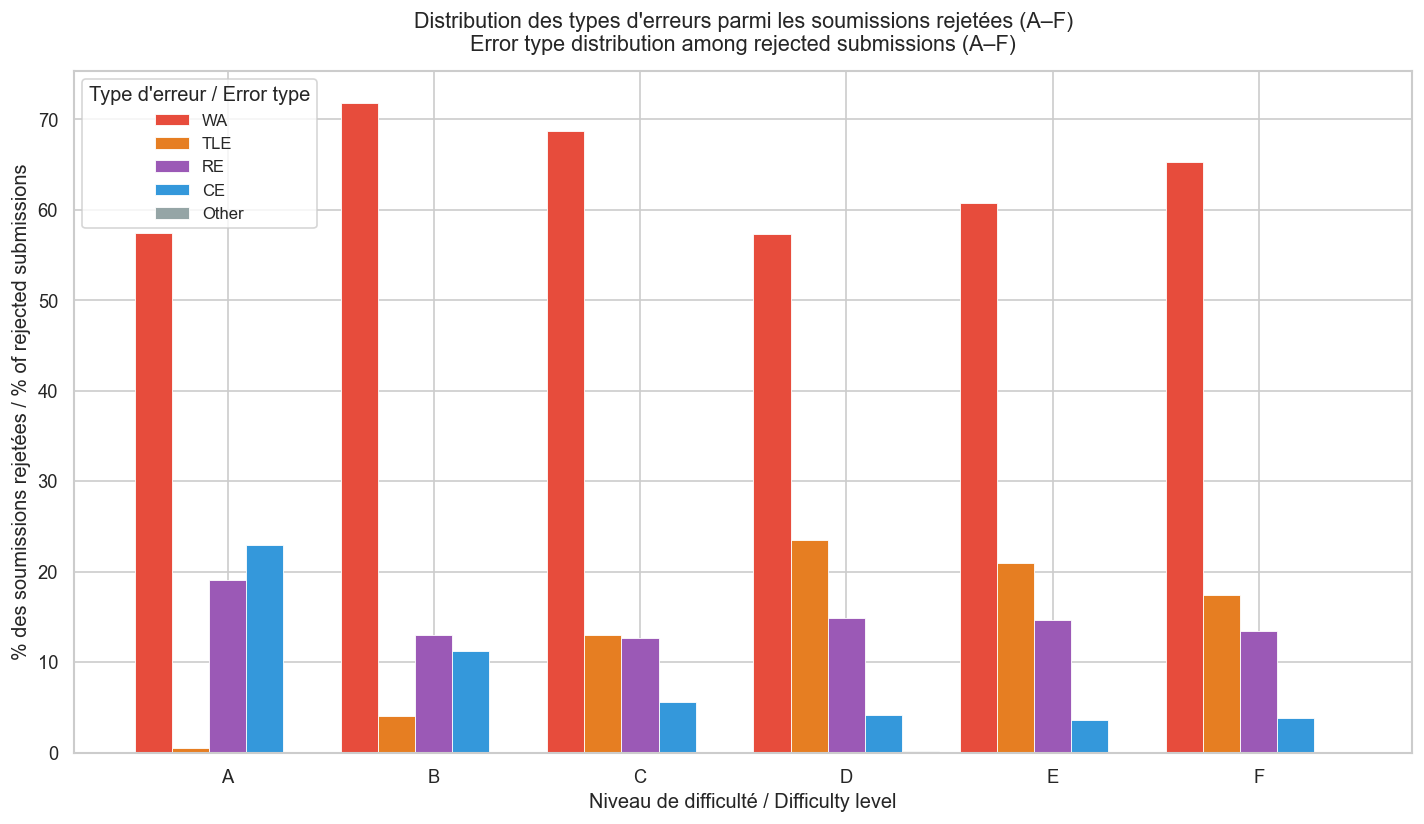
\includegraphics[height=3.1cm]{nb02_ce_tle_inversion.png}\\[1mm]
    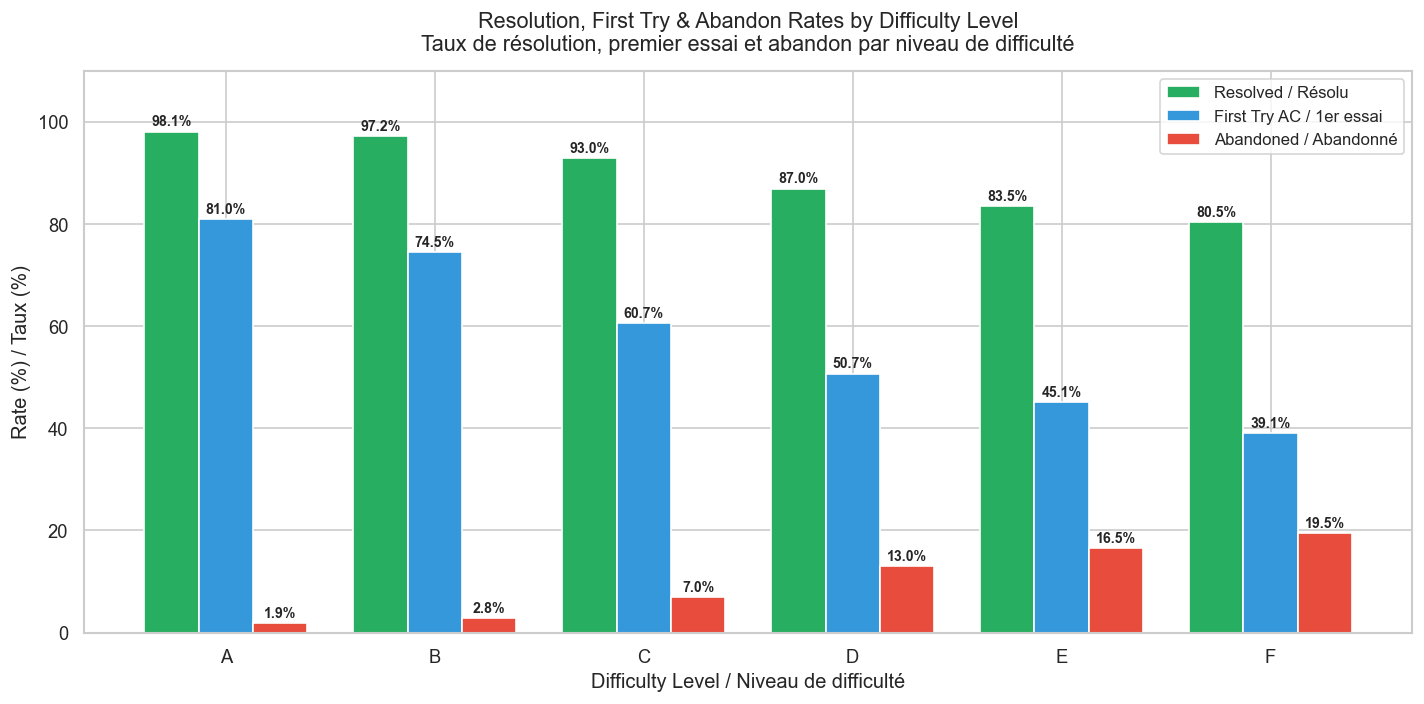
\includegraphics[height=3.1cm]{nb05_resolution_by_difficulty.png}
  \end{columns}
\end{frame}

\begin{frame}{Expertise Flattens the Effect of Error Type}
  \begin{columns}[T]
    \column{0.52\textwidth}
    \begin{itemize}
      \item \textbf{Question}: does the type of a user's first error
        predict final success, the same way for everyone?
      \item TLE = worst first-error signal, at \alert{every} level without
        exception (pooled across groups)
      \item \textbf{But} that gap depends on skill: best/worst error-type
        resolution gap --- 18pp for G4, only 3.5pp for G6 (level D)
    \end{itemize}
    \column{0.44\textwidth}
    \centering
    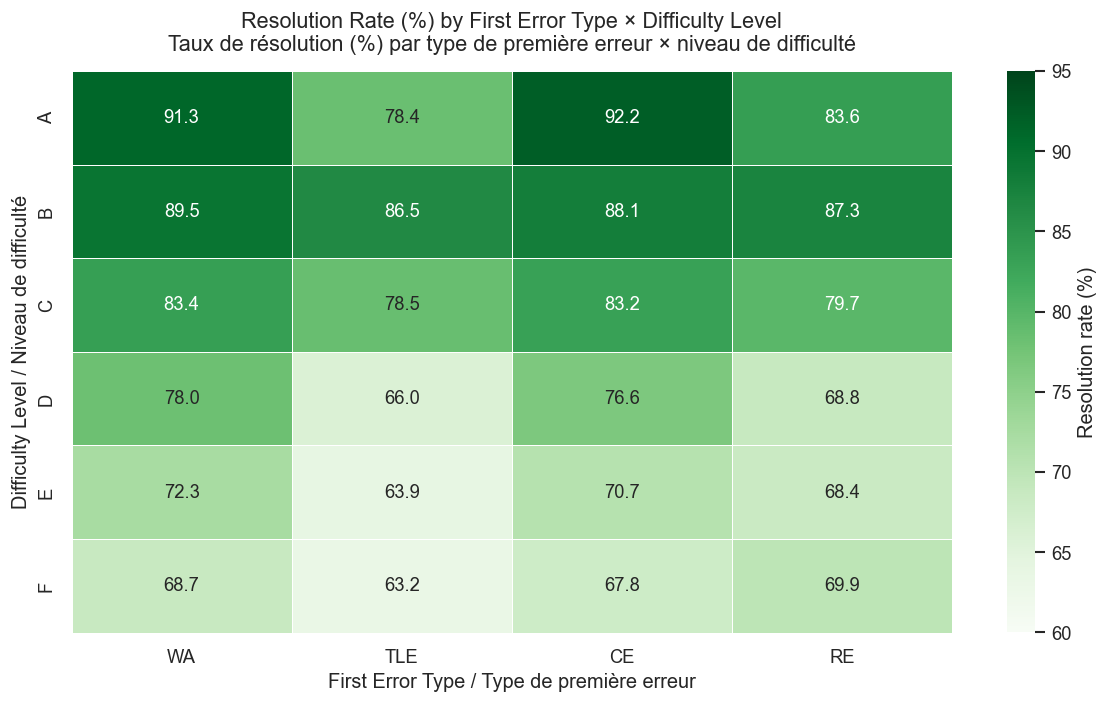
\includegraphics[height=3.0cm]{nb06_resolution_by_error_pooled.png}\\[1mm]
    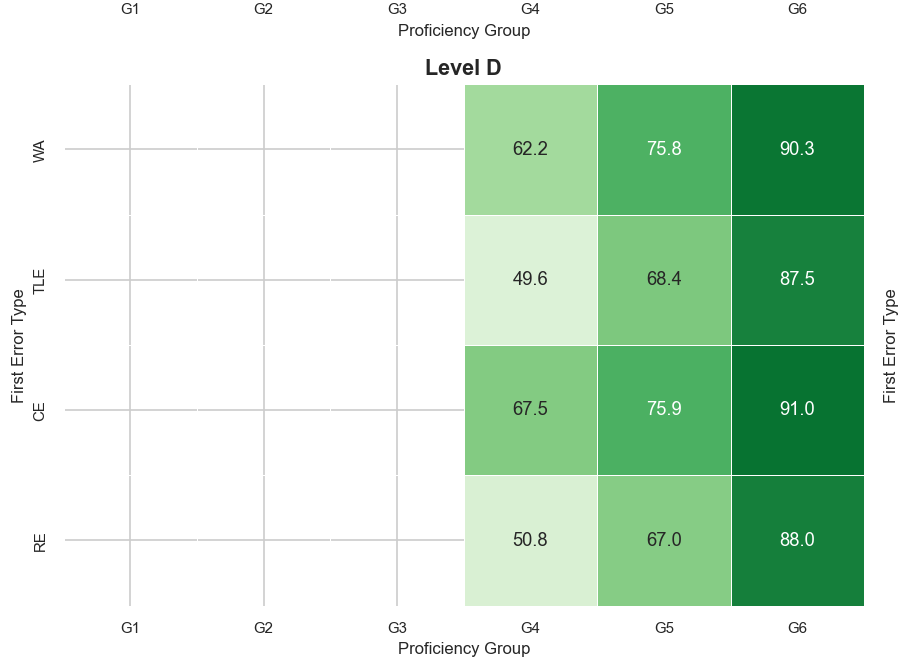
\includegraphics[height=3.0cm]{nb06_expertise_leveld.png}\\
    {\tiny\color{gray} Bottom: level D only (full grid: NB06, Sec. 4)}
  \end{columns}
\end{frame}

\begin{frame}{The \emph{Blind Patch} Anomaly}
  \begin{columns}[T]
    \column{0.52\textwidth}
    \begin{itemize}
      \item \textbf{Question}: does the delay before resubmitting after a
        TLE change the odds of success?
      \item \textbf{Result}: resubmitting within 2--5 min is \alert{worse}
        than either faster or later ($n > 37{,}000$, level D)
      \item The only result that wasn't predictable \emph{a priori} (stated
        as such in the notebook itself)
    \end{itemize}
    \column{0.44\textwidth}
    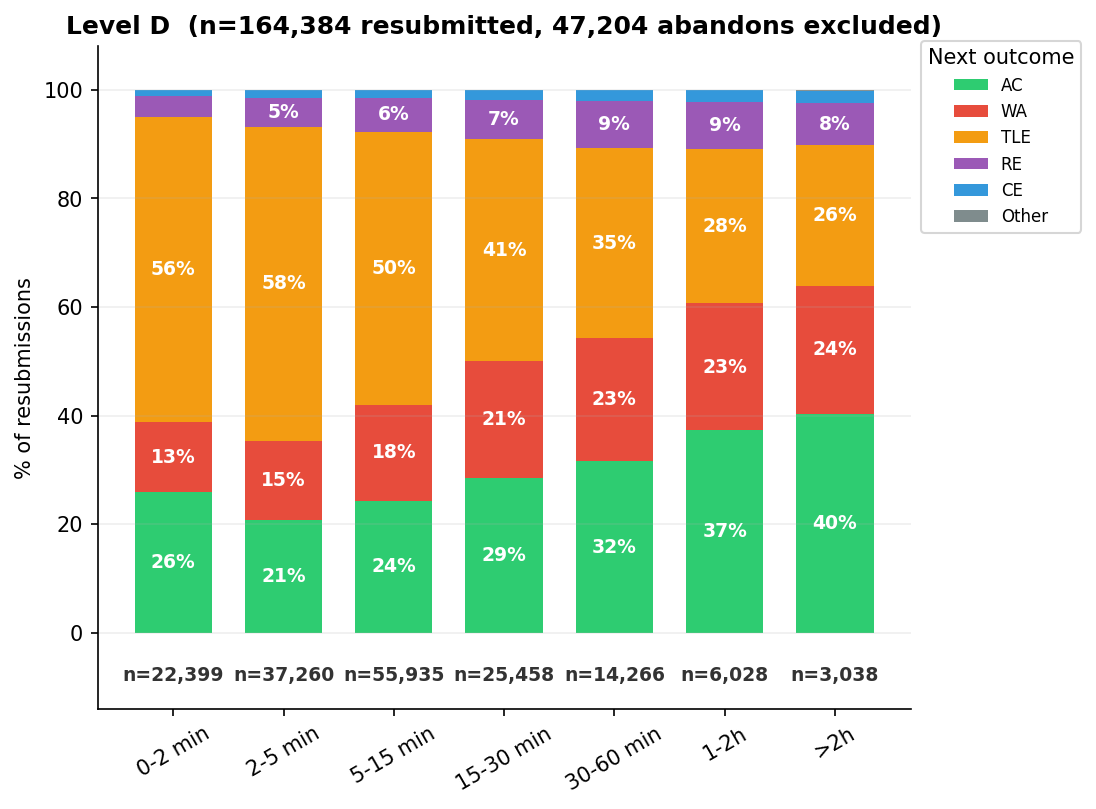
\includegraphics[width=\linewidth]{nb08_blindpatch_leveld.png}\\
    {\tiny\color{gray} Level D panel shown (NB08, S1, full grid covers all
    6 levels).}
  \end{columns}
\end{frame}

\begin{frame}{Summary --- RQ1}
  \begin{itemize}
    \item Error patterns depend on language, expertise, and even resubmission
      behavior
    \item Throughline: expertise doesn't just lower the error rate --- it
      lowers \alert{how much the error type matters}
  \end{itemize}
\end{frame}

% ═══════════════════════════════════════════════════════════════════════════
\section{Results --- RQ2}

\begin{frame}{Reminder: RQ2}
  \begin{center}
    \Large Do codes that are close together in vector space share the
    same error pattern?
  \end{center}
\end{frame}

\begin{frame}{Sanity Check: Is the Embedding Credible At All?}
  \begin{itemize}
    \item Before asking whether it captures \emph{verdict}: does the
      embedding capture \emph{anything} recognizable?
    \item \alert{Yes} --- problem identity is trivial to see; verdict is
      not, on the exact same points
  \end{itemize}
  \centering
  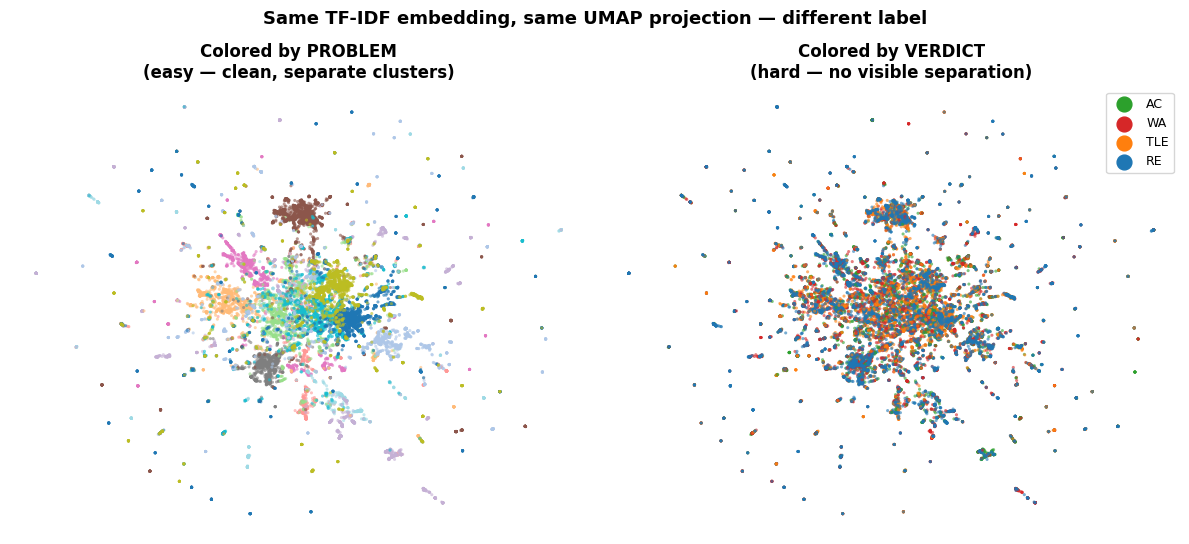
\includegraphics[width=0.9\linewidth]{nb10_umap_sanity_check.png}
\end{frame}

\begin{frame}{CodeBERT vs TF-IDF}
  \begin{columns}[T]
    \column{0.52\textwidth}
    \begin{itemize}
      \item \textbf{Question}: does a semantic embedding capture the
        code$\leftrightarrow$verdict link better than plain TF-IDF?
      \item \textbf{Method}: k-NN lift (k=10, cosine), control funnel
        language $\to$ problem $\to$ both
      \item \textbf{Result}: once fully controlled, \alert{CodeBERT
        provides no advantage} --- even in Python (×1.33 TF-IDF vs ×1.29
        CodeBERT)
    \end{itemize}
    \column{0.44\textwidth}
    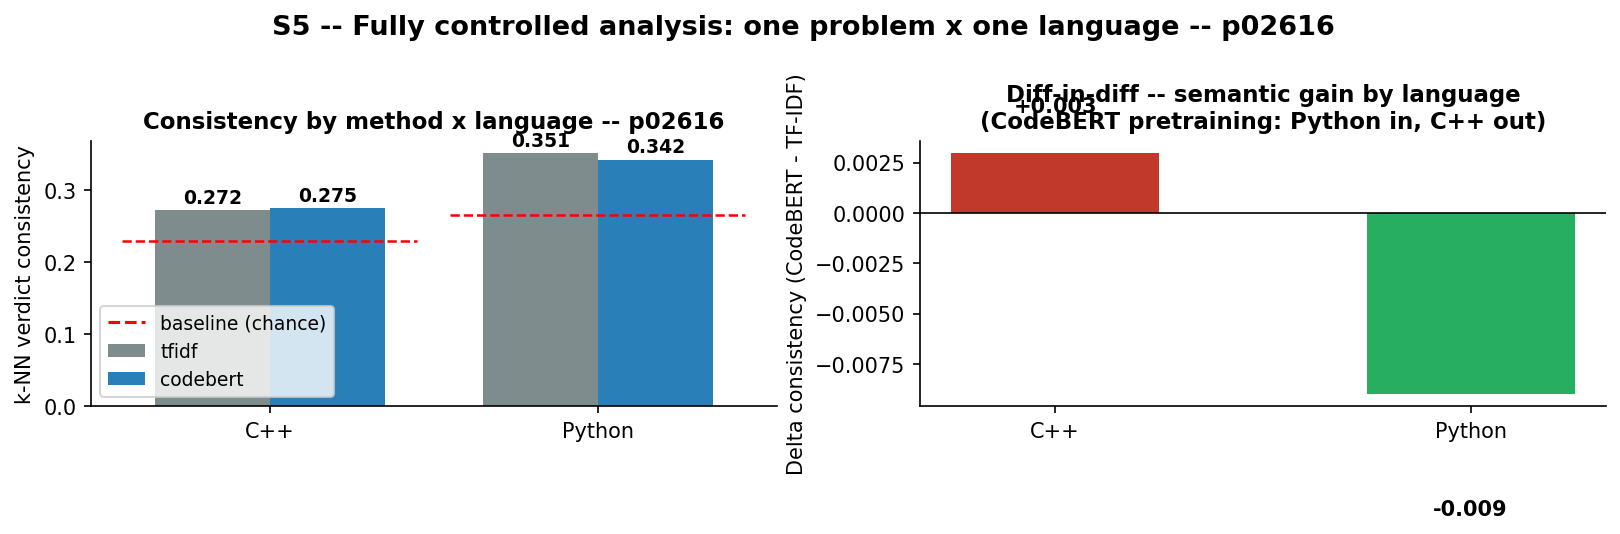
\includegraphics[width=\linewidth]{nb10_codebert_vs_tfidf.png}\\
    {\tiny\color{gray} S5, single-problem/single-language control
    (p02616). Right panel: CodeBERT $-$ TF-IDF, Python is negative.}
  \end{columns}
\end{frame}

\begin{frame}{Generalization --- and a Methodological Twist}
  \begin{columns}[T]
    \column{0.52\textwidth}
    \begin{itemize}
      \item Confirmed across 12 problems (21,773 submissions) --- on
        \alert{verdict} (the actual RQ2 question), TF-IDF and CodeBERT are
        near tied (×1.37 vs ×1.35, 7/12 vs 5/12 wins); group is where
        TF-IDF pulls ahead, 11/12
      \item \textbf{Twist}: UMAP shows \alert{no} visible separation --- but
        t-SNE + a confusion heatmap reveal a real, highly localized signal
        (AC/WA 69\%/68\% neighbor consistency, TLE nearly invisible at 3\%)
    \end{itemize}
    \column{0.44\textwidth}
    \centering
    {\scriptsize UMAP --- p02659 (TF-IDF, verdict)}\\
    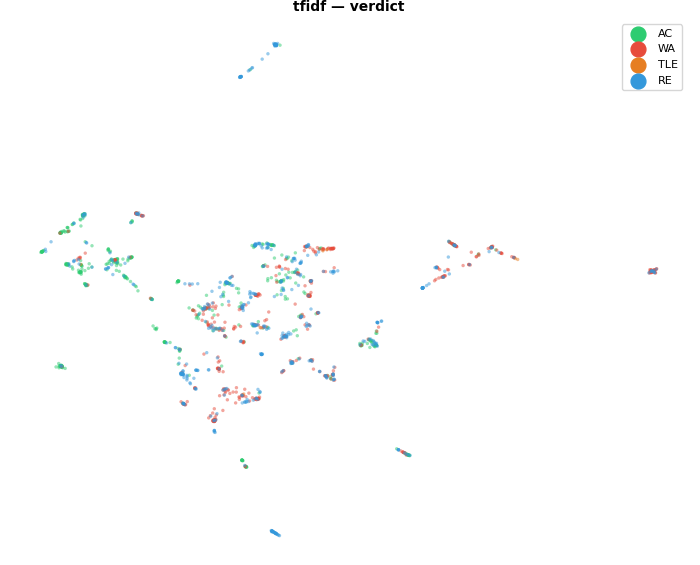
\includegraphics[height=2.75cm]{nb11_umap_p02659.png}\\[1mm]
    {\scriptsize t-SNE --- same data}\\
    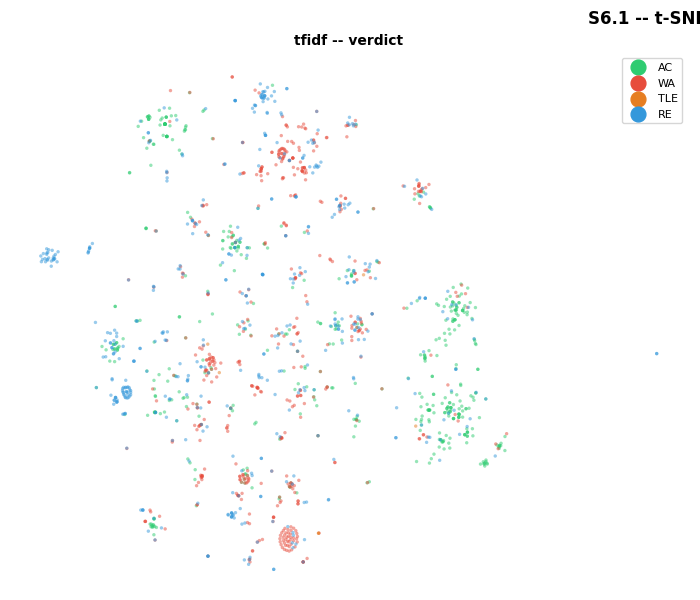
\includegraphics[height=2.75cm]{nb11_tsne_p02659.png}
  \end{columns}
\end{frame}

\begin{frame}{Zooming In --- Does Proximity Reflect Real Similarity?}
  \begin{columns}[T]
    \column{0.5\textwidth}
    \begin{itemize}
      \item \textbf{Question raised by the professors, Aug.\ 7}: do these
        clusters in the t-SNE projection reflect genuinely similar code, or
        an embedding coincidence?
      \item \textbf{Method}: automatic cluster detection (DBSCAN, not by
        eye) $\to$ real code similarity (difflib) compared to a random
        baseline of matching verdict composition
    \end{itemize}
    \column{0.48\textwidth}
    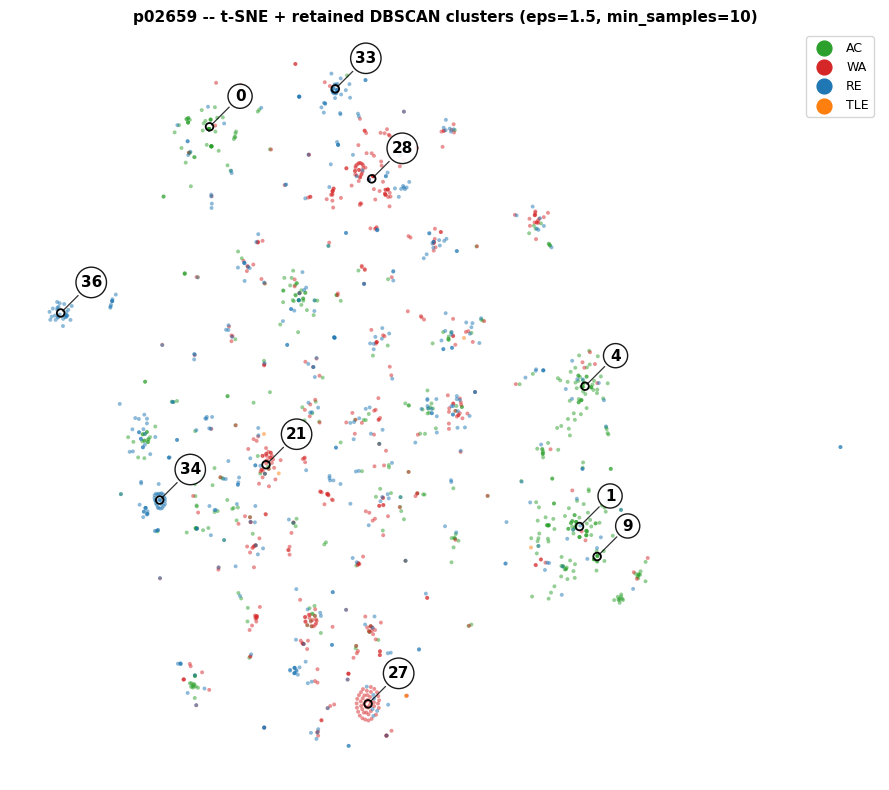
\includegraphics[width=\linewidth]{nb14_cluster_map.png}\\
    {\tiny\color{gray} 10 automatically-detected clusters, p02659 (NB14,
    S1). Numbers = cluster IDs used in the S3/S6 tables.}
  \end{columns}
\end{frame}

\begin{frame}[fragile]{Result --- the Exception Wasn't an Embedding Failure}
  \begin{columns}[T]
    \column{0.52\textwidth}
    \begin{itemize}
      \item \textbf{9/10 clusters}: code genuinely more similar than the
        baseline (up to \alert{2.73×})
      \item \textbf{Cluster 36} (0.83×, RE, 100\% pure --- the one spotted
        \emph{by eye} first): checked all 26 files, not a sample
      \item \alert{26/26 are C++}, every single one labeled ``Python'' in
        the dataset --- not the embedding failing on comparable code, a
        \alert{data-labeling bug} (NB14, S7)
    \end{itemize}
    \column{0.46\textwidth}
    \centering
    {\scriptsize\color{gray} Cluster 34 (\textcolor{teal}{2.73×}) --- s144425654 / s828321135:}\\[0.5mm]
    {\tiny\begin{verbatim}
a, b = map(int,input().split())
print(int(a*b))
a,b=map(int,input().split())
print(int(a*b))
    \end{verbatim}}

    \vspace{1mm}
    {\scriptsize\color{gray} \texttt{s392220690}, cluster 36 (\textcolor{red!70!black}{0.83×}):}\\[0.5mm]
    {\tiny\begin{verbatim}
a, b = input()
print("%lld", a * b)#include <iostream>
#include <cstdio>
...
int main() {
    ...
}
    \end{verbatim}}
  \end{columns}
\end{frame}

\begin{frame}{Pushing the Model Comparison Further}
  \begin{columns}[T]
    \column{0.42\textwidth}
    \begin{itemize}
      \item \textbf{Question}: does a model aware of code structure
        (GraphCodeBERT, real data-flow graph) do better?
      \item \textbf{Result}: mixed --- no version clearly beats TF-IDF on
        k-NN (top), but a supervised probe puts the real-graph version
        ahead on verdict (bottom)
      \item No clear winner --- an open thread for the next steps
    \end{itemize}
    \column{0.54\textwidth}
    \centering
    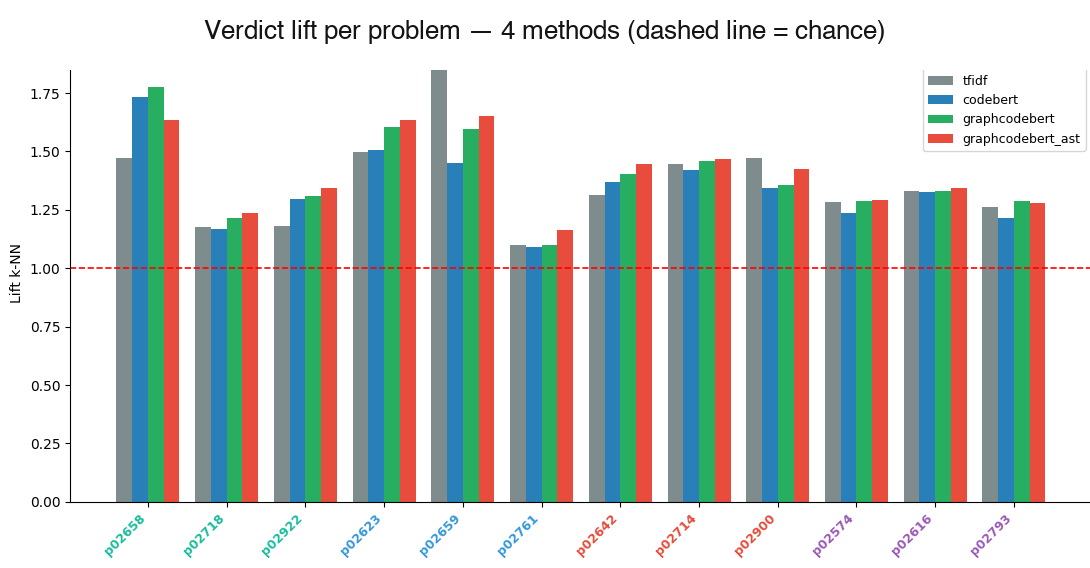
\includegraphics[width=\linewidth]{nb13_verdict_lift_4methods.png}\\[1mm]
    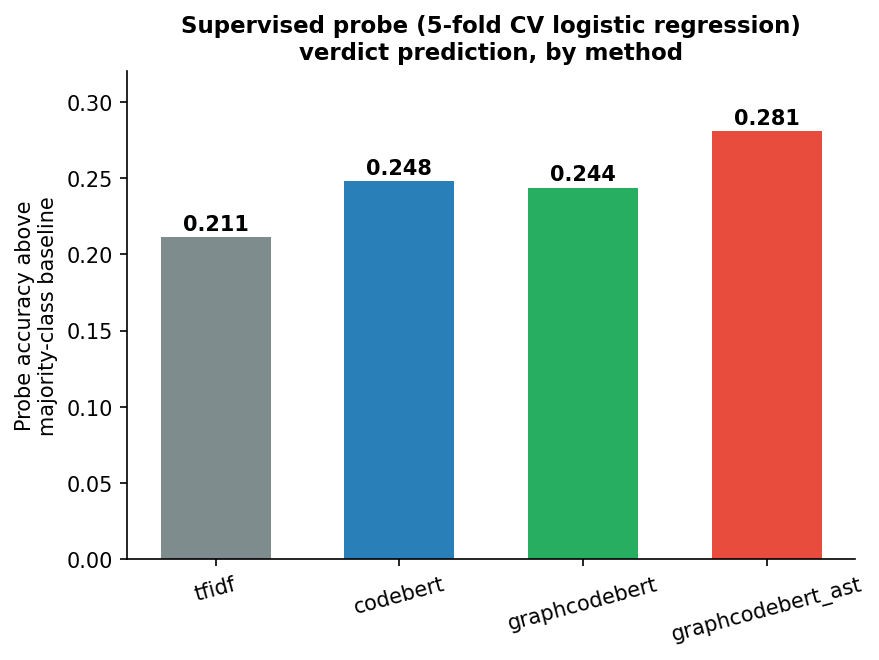
\includegraphics[height=3.4cm]{nb13_probe_verdict.png}
  \end{columns}
\end{frame}

\begin{frame}{Summary --- RQ2}
  \begin{itemize}
    \item A real but modest verdict signal, confirmed by 3 independent
      methods (k-NN lift, t-SNE+heatmap, real code via NB14)
    \item No more sophisticated model tested clearly beat TF-IDF for this
      specific task
  \end{itemize}
\end{frame}

% ═══════════════════════════════════════════════════════════════════════════
\section{Analysis and Outlook}

\begin{frame}{Summary and Next Steps}
  \begin{itemize}
    \item RQ1: rich error patterns, shaped by language, expertise, and
      resubmission behavior
    \item RQ2: a real but modest signal --- validated at the level of actual
      code, not just the embedding
    \item \textbf{Next (3 weeks after August 28)}: LLM exploration --- a
      natural direction after finding that neither CodeBERT nor GraphCodeBERT
      clearly beat TF-IDF
    \item Also on the roadmap, not started yet: RQ3 (error prediction) and
      an interactive dashboard
  \end{itemize}
\end{frame}

\begin{frame}[standout]
  Thank you!\\[2mm]
  {\large Questions?}

  \vspace{4mm}
  {\setlength{\fboxsep}{5pt}\colorbox{white}{
\includegraphics[width=2.3cm]{github_qr.png}}}\\[2mm]
  {\footnotesize\normalfont\ttfamily github.com/Raphael-Bely/OJS-submission-analytics}
\end{frame}

\end{document}
